\section{Experiments} \label{sec:exp}
A prototype\footnote{Source code available at \url{https://github.com/jgorzny/Skeptik}} version of {\FORPI} has been implemented in the functional programming language Scala as part of the \skeptik
 library. %\footnote{\url{https://github.com/Paradoxika/Skeptik}}. 
%{\SFOLowerUnits} prototype was developed earlier for the same system \cite{}.
Evaluation of this algorithm was performed on the same 308 real first-order proofs generated to evaluate {\GFOLU}, and for consistency, the same system and metrics were used (see \cite{GFOLU}).

Figure \ref{fig:ex} (a) shows the compression results of applying {\FORPI} and {\GFOLU} to the same proof (in both application orders), as well as each of these algorithms individually. 
%Unsurprisingly, applying both algorithms generally does better than either algorithm alone. 
With this data, {\FORPI} compresses provides some compression to the original proofs, although {\GFOLU} is responsible for most of the compression. {\FORPI} compresses only three proofs already compressed by {\GFOLU}.
{\RPI} performs best when the proofs are tall; {\FORPI} will likely perform similarly. However, the proofs in this data set are relatively short, and those compressed by {\GFOLU} first are even shorter. Thus, the performance of {\FORPI} is not surprising.

Figure \ref{fig:ex} (b) shows that the order of compression may matter less than in than in the propositional case, although more data is needed for confirmation. The number of points above and below the main diagonal are the same; however, the points below may simply be the result of {\GFOLU} being more likely to compress such short proofs. If so, that would imply that running {\FORPI} after {\GFOLU} is more successful, which would be consistent with propositional results for these algorithms.
%Running {\FORPI} after {\GFOLU} shows some compression that...
%This is consistent with propositional results for these algorithms.

%Before evaluating this algorithm, we first generated several benchmark proofs. This was done by executing the {\SPASS}\footnote{\url{http://www.spass-prover.org/}} theorem prover on 2280 real first-order problems without equality of the TPTP Problem Library \footnote{\url{http://www.cs.miami.edu/{\textasciitilde}tptp/}} (among them, 1032 problems are known to be unsatisfiable). In order to generate pure resolution proofs, most advanced inference rules used by {\SPASS}  were disabled. The Euler Cluster at the University of Victoria\footnote{\url{https://rcf.uvic.ca/euler.php}} was used and the time limit was 300 seconds per problem. Under these conditions, {\SPASS} was able to generate 308 proofs. 


%The proofs generated by {\SPASS} were small (with lengths from 3 to 49). These proofs are specially small in comparison with the typical proofs generated by SAT- and SMT-solvers, which usually have from a few hundred to a few million nodes. The number of proofs (compressed and uncompressed) per length is shown in Figure \ref{fig:ex} (b). Uncompressed proofs are those which had either no lowerable units to lower or for which \SFOLowerUnits failed and returned the original proof. Such failures occurred on only 14 benchmark proofs. Among the smallest of the 308 proofs, very few proofs were compressed. This is to be expected, since the likelihood that a very short proof contain a lowerable unit (or even merely a unit with more than one child) is low. The proportion of compressed proofs among longer proofs is, as expected, larger, since they have more nodes and it is more likely that some of these nodes are lowerable units. 13 out of 18 proofs with length greater than or equal to 30 were compressed. 

%Figure \ref{fig:ex} (a) shows a box-whisker plot of compression ratio with proofs grouped by length and whiskers indicating minimum and maximum compression ratio achieved within the group. Besides the median compression ratio (the horizontal thick black line), the chart also shows the mean compression ratios for all proofs of that length and for all compressed proofs (the red cross and the blue circle). In the longer proofs (length greater than 34), the median and the means are in the range from 5\% to 15\%, which is satisfactory in comparison with the total compression ratio of 7.5\% that has been measured for the propositional {\LowerUnits} algorithm on much longer propositional proofs \cite{Boudou}.

%Figure \ref{fig:ex} (c) shows a scatter plot comparing the length of the input proof against the length of the compressed proof. For the longer proofs (circles in the right half of the plot), it is often the case that the length of the compressed proof is significantly lesser than the length of the input proof.

%Figure \ref{fig:ex} (d) plots the cumulative original and compressed lengths of all benchmark proofs (for an x-axis value of $k$, the cumulative curves show the sum of the lengths of the shortest $k$ input proofs). The total cumulative length of all original proofs is 4429 while the cumulative length of all proofs after compression is 3929. This results in a total compression ratio of 11.3\%, which is impressive, considering that the inclusion of all the short proofs (in which the presence of lowerable units is a priori unlikely) tends to decrease the total compression ratio. For comparison, the total compression ratio considering only the 100 longest input proofs is 18.4\%.

%Figure \ref{fig:ex} also indicates an interesting potential trend. The gap between the two cumulative curves seems to grow superlinearly. If this trend is extrapolated, progressively larger compression ratios can be expected for longer proofs. This is compatible with Theorem 10 in \cite{LURPI}, which shows that, for proofs generated by eagerly resolving units against all clauses, the propositional {\LowerUnits} algorithm can achieve quadratic assymptotic compression. SAT- and SMT-solvers based on CDCL (Conflict-Driven Clause Learning) avoid eagerly resolving unit clauses by dealing with unit clauses via boolean propagation on a conflict graph and extracting subproofs from the conflict graph with every unit being used at most once per subproof (even when it was used multiple times in the conflict graph). Saturation-based automated theorem provers, on the other hand, might be susceptible to the eager unit resolution redundancy described in Theorem 10 \cite{LURPI}. This potential trend would need to be confirmed by further experiments with more data (more proofs and longer proofs).


%TODO: change time
%{\SPASS} required approximately 40 minutes (running on a cluster and proof generation time for each problem) to solve the generated proofs. The total time for {\GFOLU} and {\FORPI} to be executed on all 308 proofs was just under 5 seconds on a simple laptop. Both times including parsing time. These compression algorithms continue to be very fast, and may simplify the proof considerably for a relatively quick time cost.

{\SPASS} required approximately 40 minutes to solve and generate the proofs; the total time for {\GFOLU} and {\FORPI} to be executed on all 308 proofs was just under 8 seconds (both include parsing time). These algorithms are very fast, and may simplify the proof considerably for a relatively quick time cost.

\begin{figure}[bt]
\centering
    \subfloat[Compressed length against input length]{{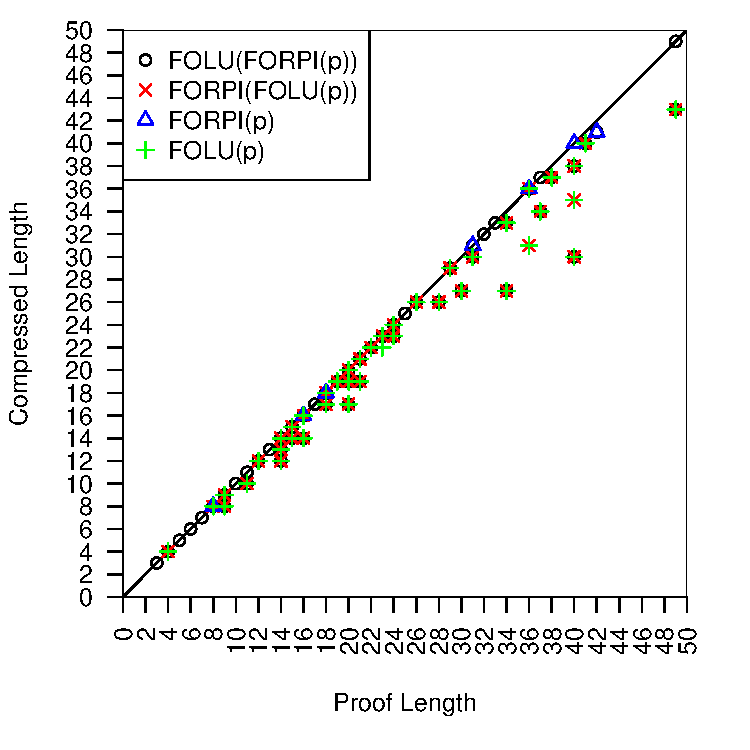
\includegraphics[scale=0.5]{images/everything-forpi-folu-length_vs_compress_length_all_proofs.pdf}}}
%    \subfloat[Compressed length against input length (resolutions)]{{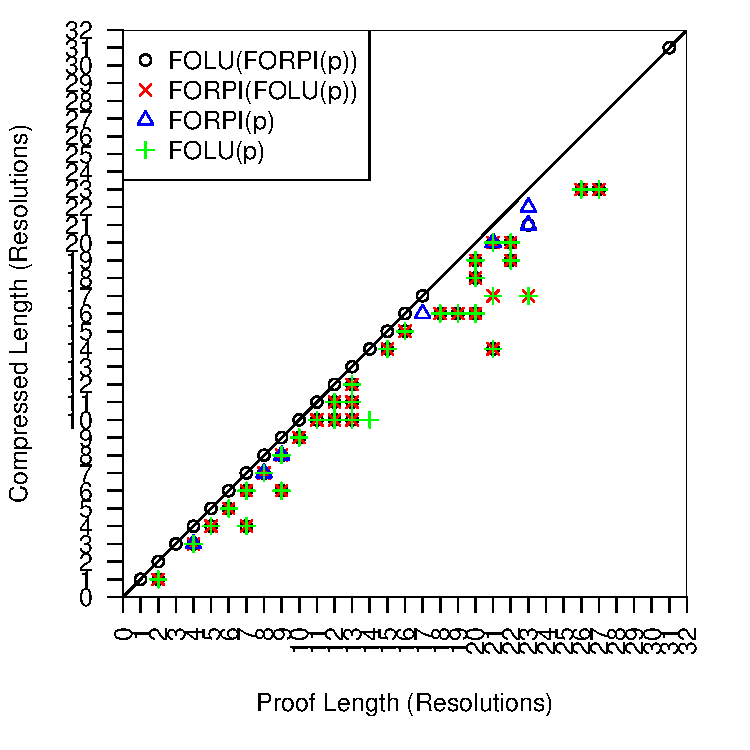
\includegraphics[scale=0.5]{images/everything-forpi-folu-res_length_vs_compress_res_length_all_proofs.pdf} }}
\subfloat[\FORPI(\GFOLU(p)) vs. \GFOLU(\FORPI(p))]{{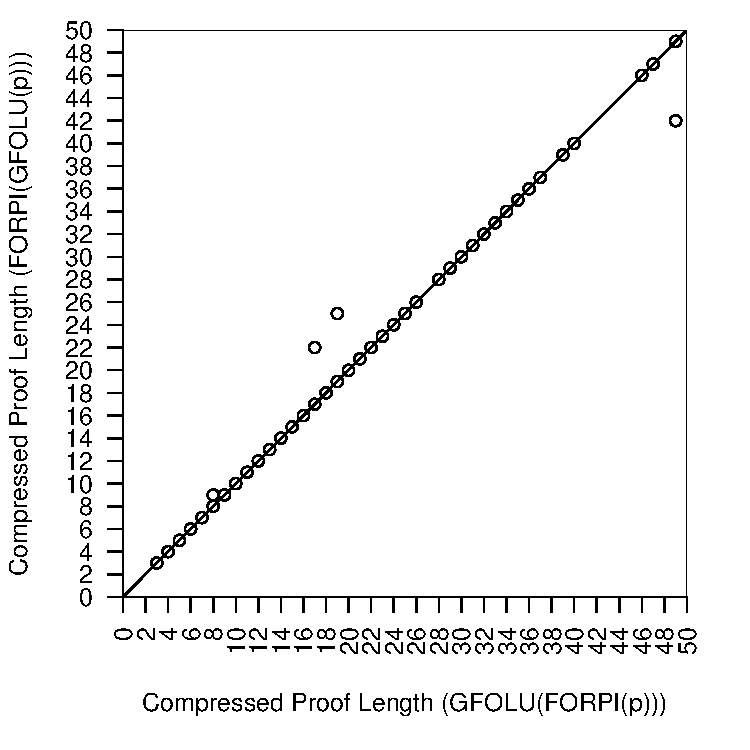
\includegraphics[scale=0.5]{images/forpi-folu-vs-folu-forpi-length_vs_compress_length_all_proofs.pdf} }}
\caption{Experimental results}
\label{fig:ex}
\end{figure}


